\documentclass[12pt, titlepage, a4paper]{article}
\usepackage[utf8]{inputenc}
\usepackage{changepage}
\usepackage{prftree}
\usepackage{amssymb}
\usepackage{amsmath}
\usepackage{enumitem} 
\usepackage{graphicx}
\usepackage{wrapfig}
\usepackage[spanish]{babel}
\usepackage{amsthm}
\usepackage{bussproofs}
\usepackage{bm}
\usepackage{url}
\usepackage{hyperref}
\usepackage{dirtytalk}

\usepackage{titlesec}
\usepackage[export]{adjustbox}

\setcounter{secnumdepth}{4}

\titleformat{\paragraph}
{\normalfont\normalsize\bfseries}{\theparagraph}{1em}{}
\titlespacing*{\paragraph}
{0pt}{3.25ex plus 1ex minus .2ex}{1.5ex plus .2ex}


\usepackage[a4paper, total={6in, 8in}]{geometry}


\usepackage{amsmath}
\usepackage{algorithm}
\usepackage{algorithmic}


\title{Introducción a la Inteligencia Artificial \\
Trabajo Práctico 2: Ontologías }
\author{Agustín Fernández Bergé y Ramiro Gatto}
\date{14/04/2025}


\begin{document}
\maketitle

\section{Introducción}
La idea de este trabajo es modelar una ontología 
(en Protege) sobre lenguajes de  
programación, en la cual se relaciones características que estos 
poseen. El principal uso de la misma es permitir ayudar a un programador
a elegir un lenguaje apropiado para un proyecto según sus necesidades. 

\section{Pasos a Seguir}
Para guiarnos en la creación de la ontología seguimos el \say{Pipeline} que 
vimos en clase, el cual consiste en lo siguientes pasos:

\begin{enumerate}
    \item {\textbf{Determinar dominio y alcance}\\
           En esta primera instancia nos planteamos preguntas que deben 
           ser respondidas por la ontología. ESte deben estar relacionadas 
           con: el dominio que cubre, el propósito de la miso, para que 
           consultas da solución. Nosotros propusimos las siguientes:
           \begin{itemize}
                \item {\say{¿Qué lenguajes funcionales tienen tipado estático y fuerte?}}
                % Berge esta lo de tipa estico y fuerte?
                \item {\say{¿Qué lenguajes tienen recolector de basura?}}
                \item {\say{¿Qué lenguajes son multiparadigmas?}} 
                \item {\say{¿Qué lenguajes son aptos para sistemas distribuidos?}}
                % Berge, al final esta pregunta la cambiamos por otra? (no mencionamos sistemas distribuidos) 
           \end{itemize}}
    \item {\textbf{Analizar Reuso}\\
           Para poder facilitar la creación de mas clases y/o tener mas 
           idea de que características usar en la ontología, una 
           forma seria viendo otras ontología ya creadas. \\

           En nuestro caso no vimos muchas ontologías ya creados y las 
           que vimos no nos terminaron de convencer.
           % Berge aca si queres podes poener lo que viste, y por que no lo usamos
           % Si usaste algo al final deci el que
           }
    \item {\textbf{Enumerar términos}\\
           En base al lo pensado en los apartados anteriores se comienza a 
           enumerar los elementos que van a aparecer en la ontología.
           Pensando:
           \begin{itemize}
            \item {¿De qué términos necesitamos hablar?}
            \item {¿Propiedades que poseen esos términos?}
            \item {¿Qué queremos decir acerca de esos términos?} 
           \end{itemize}
           Para esta ontología surgieron los siguientes (entre muchos mas):
           \begin{itemize}
            \item {Lenguajes: C, C++, Python, Haskell, ...}
            \item {Características: paradigma, gestor de memoria, forma de ejecución, ...}
           \end{itemize}}
    \item {\textbf{Definición de clases y jerarquía}\\
           Para poder definir las clases nos guiamos por la idea de que 
           una clase es una colección de elementos con propiedades 
           similares (Ejemplos de clases en esta ontología serian los 
           Lenguajes y Programas).\\

           Ademas, también se tuvo en consideración la idea 
           de subclases y superclases (Como puede ser en el caso 
           de las Características)}
    \item {\textbf{Definición propiedades de las clases (slots)}\\
           En esta sección es donde pensamos las propiedades (slots) 
           que van a tener las instancia de una clase y como 
           se van a relacionar con las instancias de otra clase. 
           Un ejemplo seria:
           \begin{enumerate}
                \item {Cada Programa fue escrito en algún Lenguaje}
                \item {Cada Lenguaje tiene algún paradigma}
           \end{enumerate}}
    \item {\textbf{Restricción de Propiedades}\\
          Es este sección, se establecieron los posibles valores de 
          los slots teniendo se: 
          \begin{itemize}
            \item {Un lenguaje de programación es una instancia de Lenguaje}
            \item {Un programa puede ser escrito por multiples lenguajes}
            \item {Los Lenguaje tienen una sola forma de gestión de memoria}
          \end{itemize}
          %Berge aca no estoy seguro que mas poner y hacer en Protege
          }
    \item {\textbf{Crear instancia}\\
         Para esta sección simplemente creamos las instancia en las 
         distintas clases y le asignamos los valores según las slots.\\ 
         Un ejemplo de esto seria, en Lenguaje agregamos la 
         instancia \textbf{C}, en GestionMemoria \textbf{Manual}. 
         Luego podemos relacionar \textbf{C} y \textbf{Manual} mediante la 
         propiedad \textbf{tieneGestionMemoria}}
\end{enumerate}

\section{Conceptos representados}
En la ontología final representamos los siguientes conceptos
\begin{itemize}
    \item {Características, cualidades que cumplen los lenguajes de programación, 
        nosotros optamos pos usar:
        \begin{itemize}
            \item {Gestión de memoria, representa las forma en las que los 
                lenguaje manejan el uso de la memoria}
            \item {Forma de ejecución, }
            \item {Paradigma, con paradigma nos referimos al
                enfoque para crear programs}
            \item {Sistema de tipo, esta clasificación se divide en 3 mas
                Chequeo de tipo (forma de verificar las signaturas de las 
                estructuras), Declaración de tipo (..), Seguridad de tipo 
                (..)}
        \end{itemize}}
    \item {Lenguajes, hace referencia a todos los lenguajes de programación 
        que decidimos agregar}
\end{itemize}

\noindent Quedándonos la siguiente ontología:
\begin{figure}[H]
    \centering
    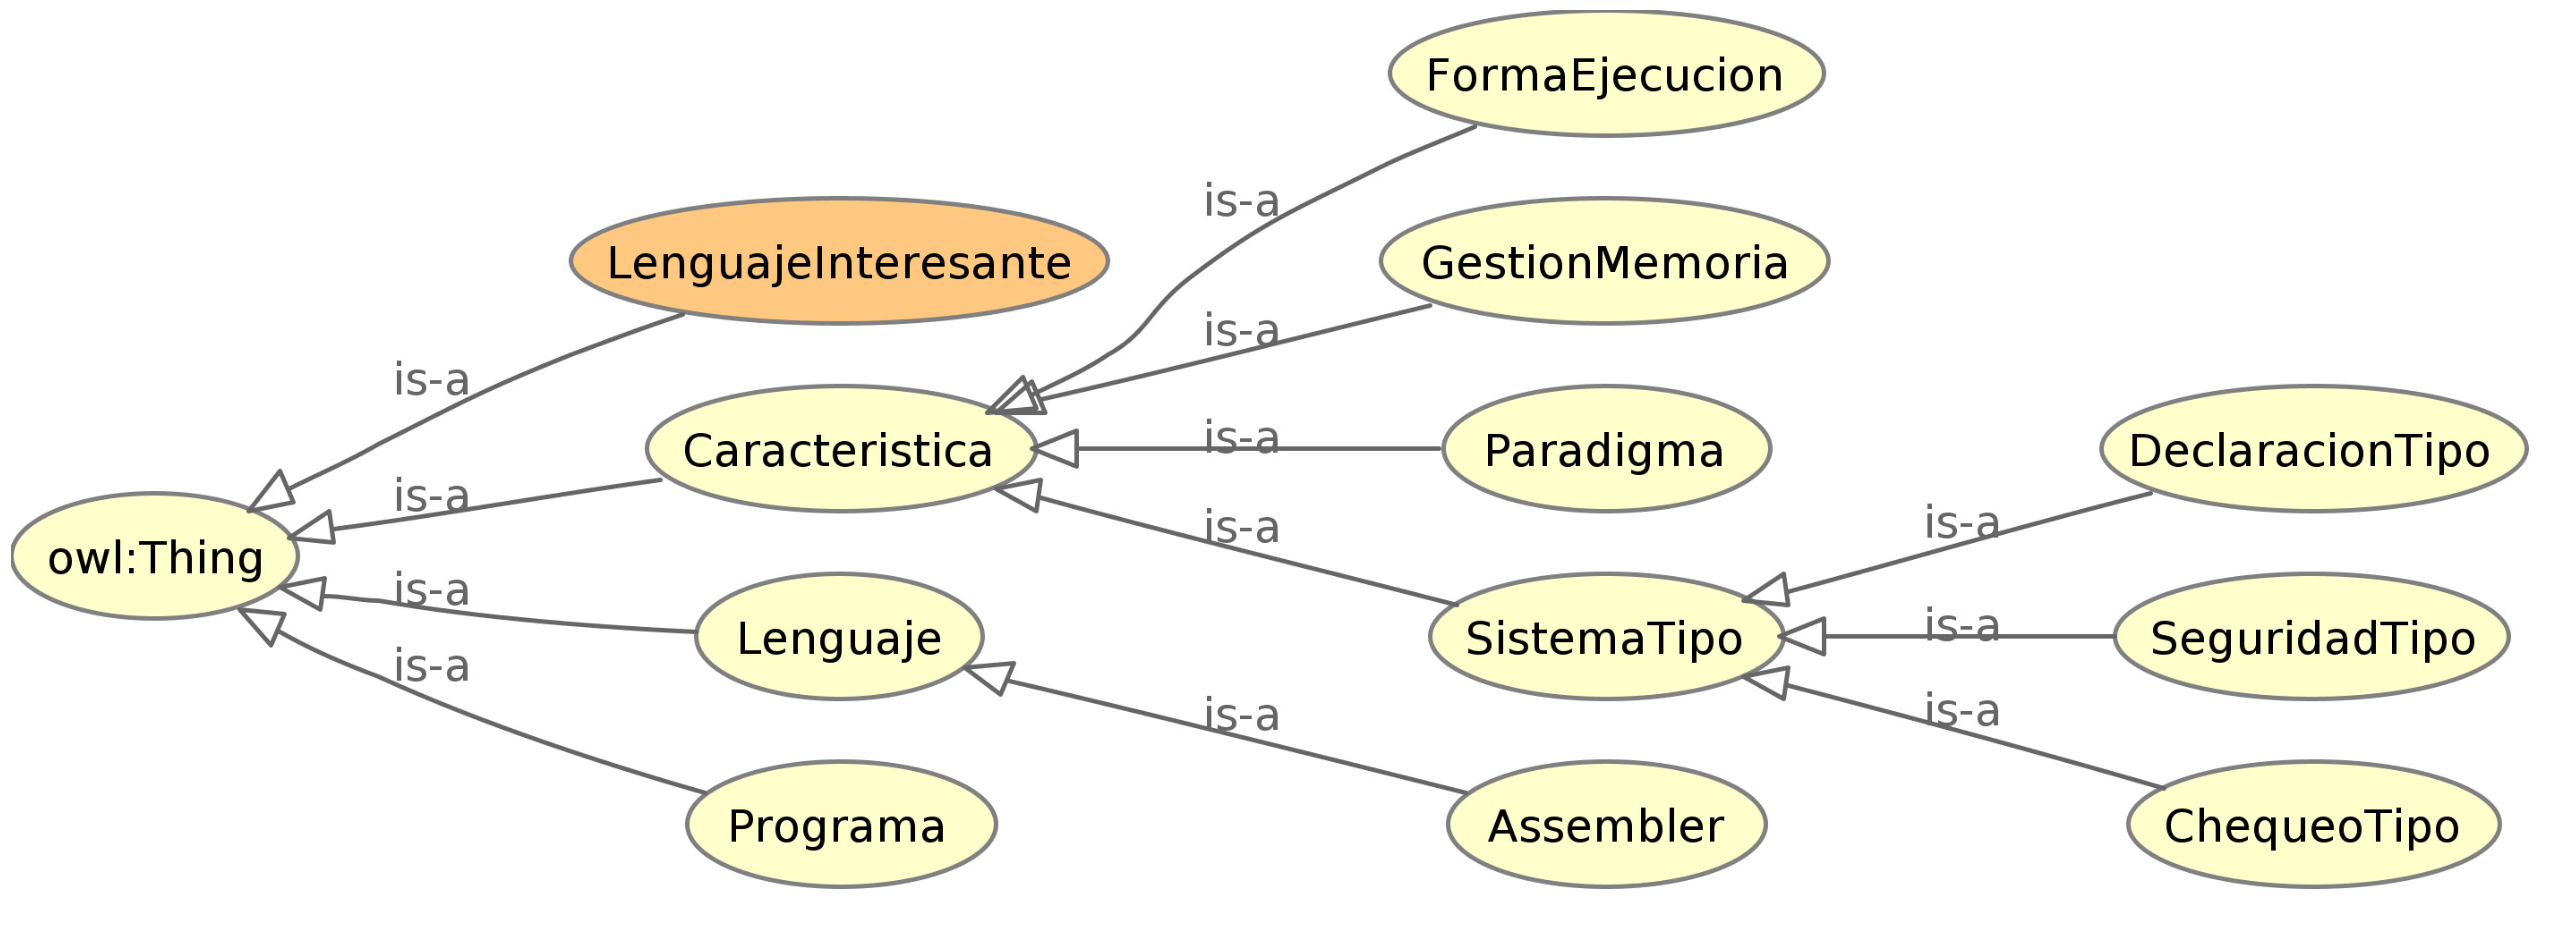
\includegraphics[width=.8\textwidth]{Imagenes/Ontologia.png}
    \caption{Ontología}
\end{figure}

\section{Instancias propuesta}
Las instancias nos quedaron de la siguiente forma:
\begin{figure}[H]
    \centering
    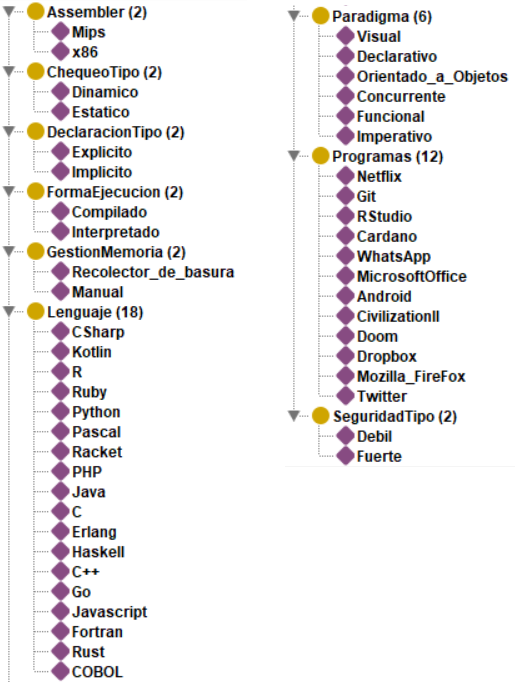
\includegraphics[width=.5\textwidth]{Imagenes/Instancias.png}
    \caption{Instancia}
\end{figure}

En cuanto al temas de las relaciones tenemos las siguientes
\begin{figure}[H]
    \centering
    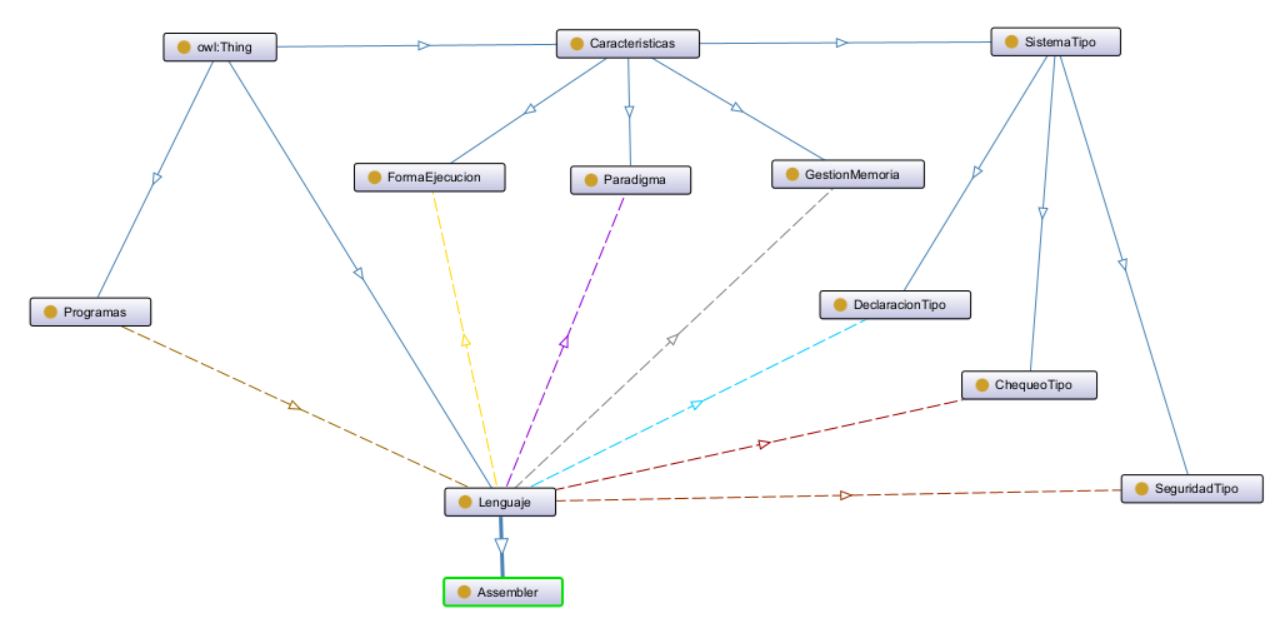
\includegraphics[width=.8\textwidth]{Imagenes/Relaciones.png}
    \caption{Relaciones, las inversas no aparecen}
\end{figure}

\section{Resultados obtenidos con el razonador}
Para ver como funciona el razonador lo que hacemos es lo siguiente, 
definimos cada relación y su inversa. Cuando \say{Instanciamos} solo 
lo hacemos con las normales, no con la inversa. De esta forma el 
razonador infiere el tipo de la inversa.\\

La otra que hacemos es dejar que intuya solo el valor de la inversa, 
es decir si las instancias A y B se relaciona mediante la realización 
f (A $\rightarrow^f$ B) dejamos que el razonador haga la inversa 
(es decir, B $\rightarrow^{f^{-1}}$ A)

%Berge, no se que mas poner

\section{Consultas realizadas}
Para ver el resultado de las consultas vamos a probar con las 
preguntas que planteamos al momento de determinar el alcance y 
veamos si en efecto es correcto.
\begin{enumerate}
    \item {La primer pregunta era: 
        ¿Qué lenguajes funcionales tienen tipado estático y fuerte?\\
        
        Usando \textbf{DL Query} escribimos la consulta, la cual tiene 
        la siguiente forma: (tieneParadigma value Funcional) and 
        (tieneSeguridadTipo value Fuerte) and 
        (tieneChequeoTipo value Estatico)\\

        Obteniéndose la lista de los siguientes lenguajes: C++, CSharp, 
        Fortran, Haskell, Java, Kotlin y Rust.

        Los cuales en efecto cumplen con lo pedido.
        }
    %Berge, falta completar con las otras preguntas
\end{enumerate}


\section{Análisis del razonamiento del razonador}
%Ni la mas puta idea


\section{Conclusion}
Durante la creación de la ontología surgieron muchas cuestión en el 
aspecto de como plantearla, en un inicio, por ejemplos, iban a poner 
los lenguajes como clases y las instancias de las misma iban a ser la 
distintas version. Pero esta idea se nos resulto muy complejo 
(lo mismo, íbamos a hacer con las instancias de las subclases de 
la clase Característica).

%Berge agrega cosas que no pudiste hacer y el porque

\end{document}